\documentclass{ximera}

%\addPrintStyle{..}

\begin{document}
	\author{Bart Lambregs}
	\xmtitle{Begrippen}{}
    \xmsource\xmuitleg




	%%%\section{Enkele begrippen}

	\subsection{Plaats, verplaatsing, afgelegde weg, acceleratie}
	
	Om aan een vectoriële snelheid te komen, voeren we een plaatsvector $\vec{r}$ in. Deze kan van de tijd afhangen en kunnen we met behulp van de eenheidsvectoren $\vec{e}_x$ en $\vec{e}_y$ schrijven als
	\begin{equation*}
	 \vec{r}=x\cdot\vec{e}_x+y\cdot\vec{e}_y.
	\end{equation*}
	De tijdsafhankelijkheid kunnen we expliciet weergeven door $x(t)$ en $y(t)$ te gebruiken i.p.v. $x$ en $y$. De functies $x(t)$ en $y(t)$ noemen we de \emph{coördinaat\-functies}. Door de plaats met een vector te beschrijven, kunnen we het begrip verplaatsing $\Delta x$ ook gemakkelijk en analoog uitbreiden naar twee dimensies. De verplaatsing
	\begin{equation*}
	\Delta\vec{r}=\vec{r}_2-\vec{r}_1
	\end{equation*}
	is nu immers ook een vector die naast de afstand in vogelvlucht tussen twee punten, ook ge\"oriënteerd is. Het is natuurlijk belangrijk in welke richting die afstand wordt afgelegd.
	\begin{image}
	
	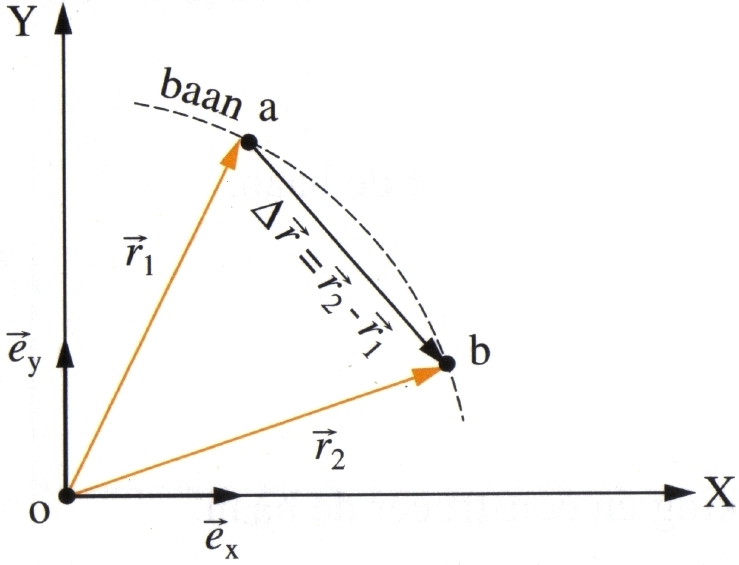
\includegraphics[width=0.4\textwidth]{plaatsvector}
	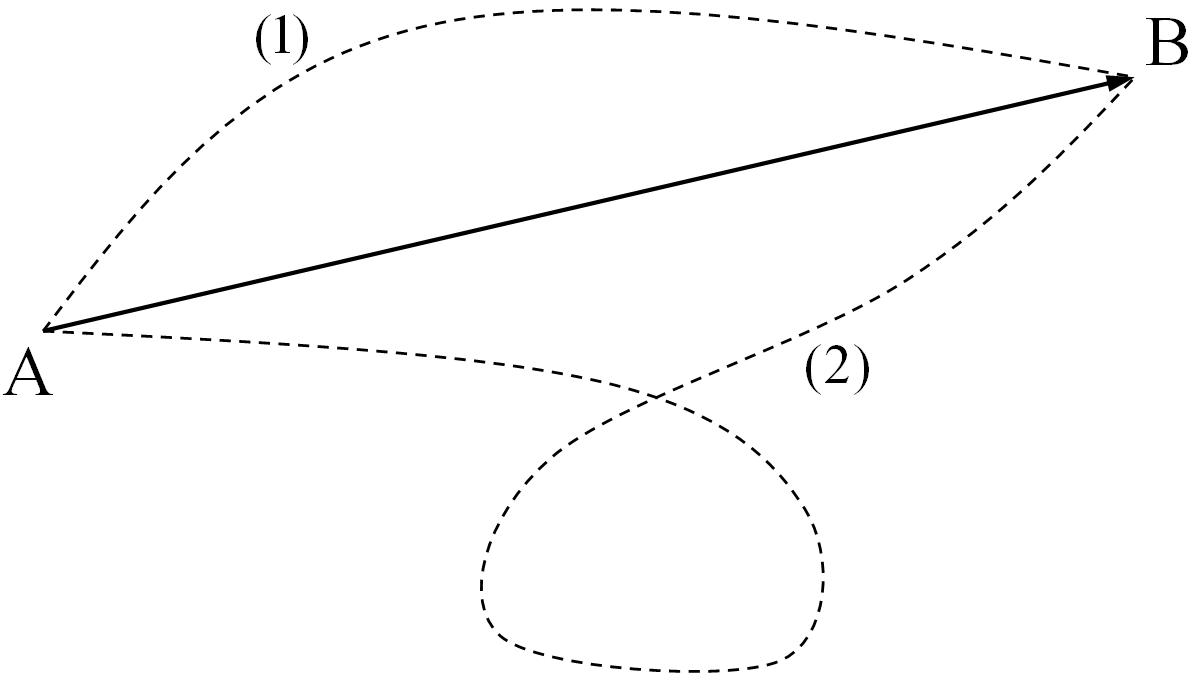
\includegraphics[width=0.4\textwidth]{afgelegdeweg_verplaatsing}
	\end{image}
	\captionof{figure}{Het verschil tussen afgelegde weg en verplaatsing}
	Merk op dat de begrippen verplaatsing en afgelegde weg niet hetzelfde zijn. De afgelegde weg hangt af van de gevolgde baan en is de totale afgelegde afstand terwijl de verplaatsing enkel van begin- en eindpunt afhangt en een vectorgrootheid is.
	
	Naast de coördinaatfuncties $x(t)$ en $y(t)$ is er ook de vergelijking van de baan $y(x)$. We bekomen deze door de tijd uit de coördinaatfuncties te elimineren\footnote{Dit komt neer op de inverse $t(x)$ van $x(t)$ te vinden en deze te substitueren in $y(t)$. Dus $y(x)=y(t(x))$.}. De grafiek van deze baanvergelijking geeft ons het beeld van de baan maar zegt niets over de snelheid waarmee het object over deze baan beweegt. Daarvoor hebben we de afhankelijkheid van de tijd nodig.
	
	\subsection{Snelheid}
	
	%\begin{wrapfigure}[9]{R}{0.35\textwidth}
	%
	%\includegraphics[width=0.34\textwidth]{snelheidsvector}
	%\end{wrapfigure}
	Analoog aan de snelheid in één dimensie, kunnen we in meerdere dimensies de snelheid definiëren als de afgeleide -- nu van de plaatsvector. De snelheid is dan opnieuw een vector:\footnote{De definitie van een afgeleide van een vector is evenzeer met een limiet. We maken gebruik van de uitdrukkingen $\vec{r}(t+\Delta t)=x(t+\Delta t)\vec{e}_x+y(t+\Delta t)\vec{e}_y$ en $\vec{r}(t)=x(t)\vec{e}_x+y(t)\vec{e}_y$.\begin{eqnarray*}
	\vec{v}=\frac{d\vec{r}}{dt}&=&\lim_{\Delta t\to 0}\frac{\vec{r}(t+\Delta t)-\vec{r}(t)}{\Delta t}\\
	&=&\lim_{\Delta t\to 0}\frac{[x(t+\Delta t)\vec{e}_x+y(t+\Delta t)\vec{e}_y]-[x(t)\vec{e}_x+y(t)\vec{e}_y]}{\Delta t}\\
	&=&\lim_{\Delta t\to 0}\frac{[x(t+\Delta t)-x(t)]\vec{e}_x+[y(t+\Delta t)-y(t)]\vec{e}_y}{\Delta t}\\
	&=&\lim_{\Delta t\to 0}\left(\frac{x(t+\Delta t)-x(t)}{\Delta t}\right)\vec{e}_x+\lim_{\Delta t\to 0}\left(\frac{y(t+\Delta t)-y(t)}{\Delta t}\right)\vec{e}_y\\
	&=&\frac{dx}{dt}\vec{e}_x+\frac{dy}{dt}\vec{e}_y%\\&=&v_x\vec{e}_x+v_y\vec{e}_y
	\end{eqnarray*}}
	\begin{eqnarray*}
	\vec{v}=\frac{d\vec{r}}{dt}=\frac{d}{dt}\left(x\cdot\vec{e}_x+y\cdot\vec{e}_y\right)=\frac{dx}{dt}\vec{e}_x+\frac{dy}{dt}\vec{e}_y%=v_x\vec{e}_x+v_y\vec{e}_y
	\end{eqnarray*}
	De eenheidsvectoren $\vec{e}_x$ en $\vec{e}_y$ veranderen niet in de tijd zodat we die buiten de afgeleide hebben kunnen brengen. We zien dat de snelheidsvector dus te ontbinden is in componenten waarbij de componenten gewoonweg de snelheden van de afzonderlijke coördinaten zijn. 
	\begin{eqnarray*}
	\vec{v}=v_x\vec{e}_x+v_y\vec{e}_y\quad\mathrm{met}\quad v_x=\frac{dx}{dt},\,v_y=\frac{dy}{dt}
	\end{eqnarray*}
	
	%\begin{image}
	%
	%%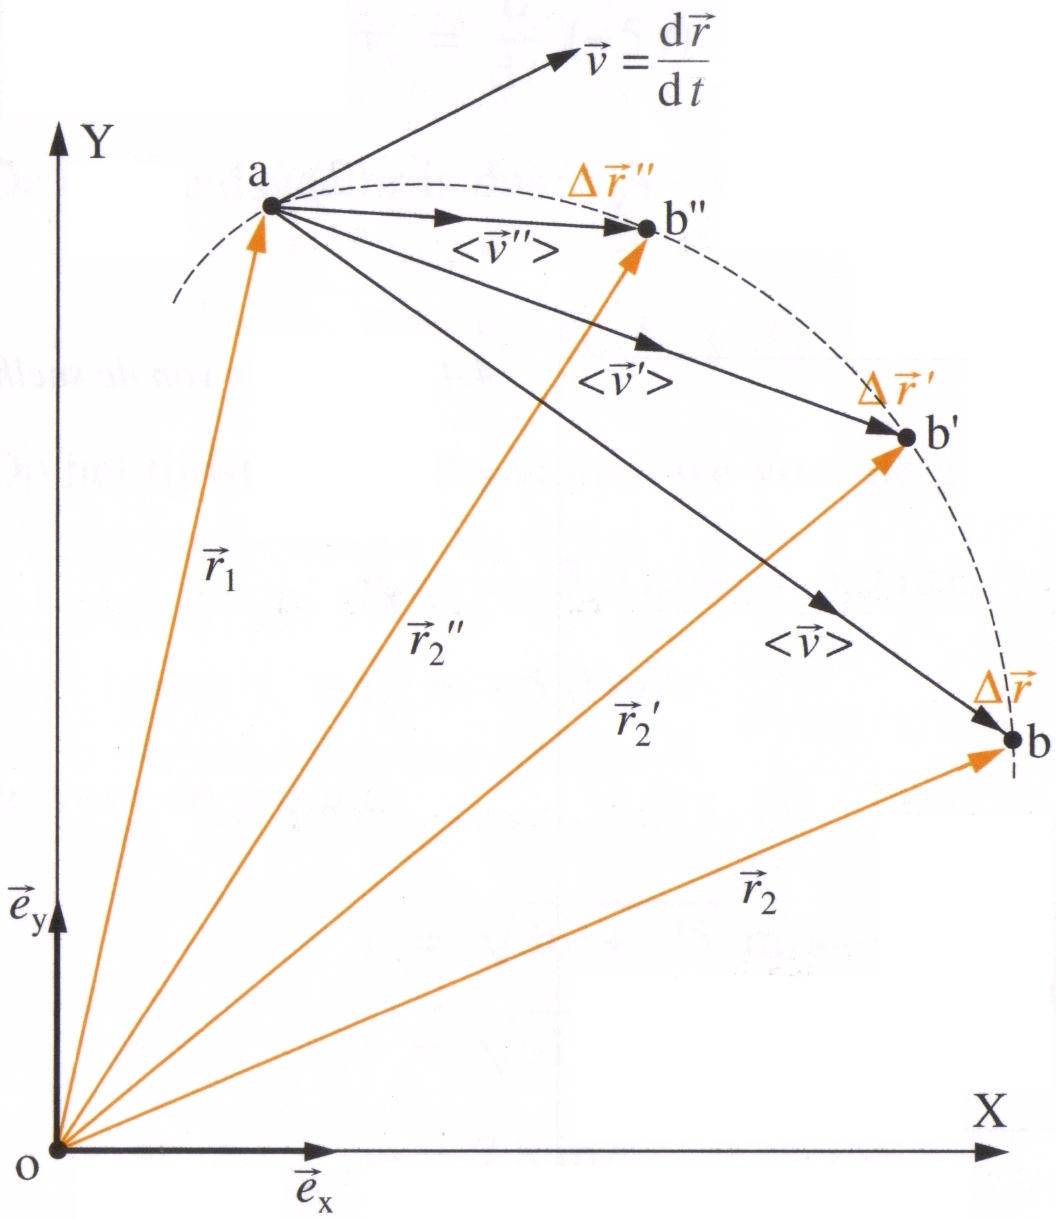
\includegraphics[width=0.38\textwidth]{gem_snelheidsvector}
	%%\hspace{1cm}
	%\includegraphics[width=0.4\textwidth]{snelheidsvector}
	%\captionof{figure}{De snelheidsvector is te ontbinden in componenten}
	%\end{image}
	%%%%\newline
	
	%%\newpage
	
	\begin{eigenschap}
	De snelheidsvector is rakend aan de baan.
	\end{eigenschap}
	%\begin{image}
	%
	%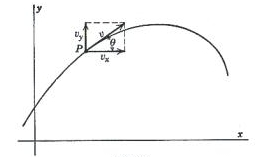
\includegraphics[width=0.4\textwidth]{snelheidrakend}
	%\captionof{figure}{De snelheid raakt aan de baan}
	%\end{image}
	\begin{proof}
	We kunnen dit bewijzen met de kettingregel, toegepast op de functie $y(t)=y(x(t))$.
	\begin{eqnarray*}
	 \frac{dy}{dt}=\frac{dy}{dx}\frac{dx}{dt}\Leftrightarrow\frac{dy}{dx}=\frac{\frac{dy}{dt}}{\frac{dx}{dt}}=\frac{v_y}{v_x}
	\end{eqnarray*}
	Inderdaad, $\frac{dy}{dx}$ is de helling van de baan en deze valt samen met de helling die de snelheidsvector maakt $\frac{v_y}{v_x}$.
	\end{proof}
	
	\subsection{Versnelling}
	
	Ook de versnelling definieren we analoog; als afgeleide van de snelheid.
	\begin{eqnarray*}
	\vec{a}=\frac{d\vec{v}}{dt}=\frac{dv_x}{dt}\vec{e}_x+\frac{dv_y}{dt}\vec{e}_y=a_x\vec{e}_x+a_y\vec{e}_y
	\end{eqnarray*}
	Merk op dat er een versnelling kan zijn wanneer de snelheidsvector van grootte verandert maar \'o\'ok wanneer de snelheidsvector van richting verandert! Als de snelheidsvector immers van richting verandert, veranderen zijn coördinaten $v_x$ en/of $v_y$. Merk bovendien op dat de versnelling niet noodzakelijk samen hoeft te vallen met de baan \ldots
	\begin{image}
	
	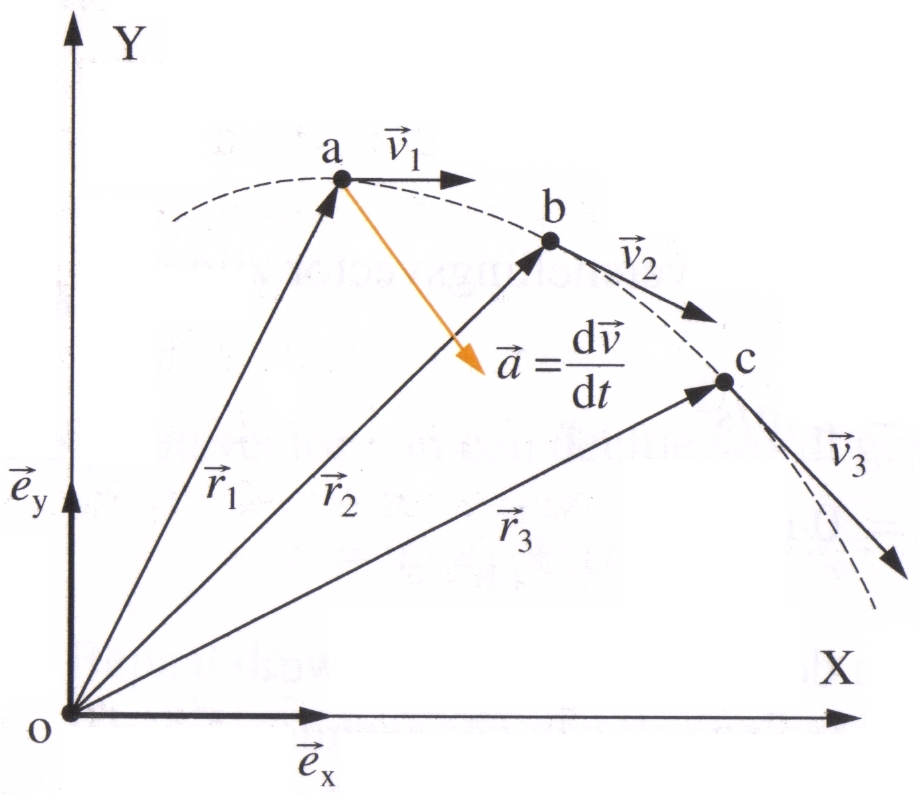
\includegraphics[width=0.4\textwidth]{versnellingsvector}
	\end{image}
	\captionof{figure}{De versnelling raakt niet noodzakelijk aan de baan}
	
	%%\newpage
	
	%oefening baanvergelijking, enz.
	
	\begin{enumerate}
	\item[\textbf{Opdracht}]\textsf{De positie van een deeltje als functie van de tijd wordt beschreven door
	\begin{displaymath}
	\vec{r}=bt\vec{e}_x+(c-dt^2)\vec{e}_y
	\end{displaymath}
	met $b=2,00\rm\,m/s$, $c=5,00\rm\,m$ en $d=1,00\rm\,m/s^2$.
	\begin{enumerate}
	\item Druk $y$ uit in functie van $x$. Hoe ziet de baan eruit?
	\item Bepaal de snelheidsvector.
	\item Op welk tijdstip ($t>0$) staat de snelheid loodrecht op de plaatsvector?
	\end{enumerate}
	\item[\textit{oplossing}]
	\begin{enumerate}
	\item We moeten dus de baanvergelijking geven. Dit doen we door de tijd uit te drukken i.f.v. de positie $x$ en dit te substitueren in de coördinaatvergelijking $y(t)$.
	\begin{eqnarray*}
	x&=&bt\Leftrightarrow t=\frac{x}{b}\\
	&\Downarrow&\\
	y&=&c-dt^2=c-\frac{d}{b^2}x^2
	\end{eqnarray*}
	Dit is een bergparabool met top $(0,c)=(0,5,00\rm\,m)$
	\item De componenten van de snelheid zijn:
	\begin{eqnarray*}
	v_x&=&\frac{dx}{dt}=b\\
	v_y&=&\frac{dy}{dt}=-2dt
	\end{eqnarray*}
	zodat de snelheid(svector) wordt gegeven door
	\begin{eqnarray*}
	\vec{v}&=&v_x\vec{e}_x+v_y\vec{e}_y\\
	&=&b\vec{e}_x-2dt\vec{e}_y
	\end{eqnarray*}
	\item De rechte die de richting van de snelheid weergeeft, staat loodrecht op de rechte die de richting van de positievector weergeeft wanneer het product van de richtingscoöefficiënten gelijk is aan $-1$:
	\begin{eqnarray*}
	rc_{r}\cdot rc_{v}&=&-1\\
	&\Updownarrow&\\
	\frac{y}{x}\cdot\frac{v_y}{v_x}&=&-1\\
	&\Downarrow&\\
	\frac{c-dt^2}{bt}\cdot\frac{-2dt}{b}&=&-1\\
	&\Downarrow&(t>0)\\
	t&=&\sqrt{\frac{2cd-b^2}{2d^2}}\\
	&=&1,73\rm\,s
	\end{eqnarray*}
	\end{enumerate}}
	\end{enumerate}
	
	%%\newpage
	
	
	
\end{document}